%%%%%%%%%%%%%%%%%%%%%%%%%%%%%%%%%%%%%%%%%%%%%%%%%%%%%%%%%%%%%%%%%%%%%
%% This is a (brief) model paper using the achemso class
%% The document class accepts keyval options, which should include
%% the target journal and optionally the manuscript type.
%%%%%%%%%%%%%%%%%%%%%%%%%%%%%%%%%%%%%%%%%%%%%%%%%%%%%%%%%%%%%%%%%%%%%
\documentclass[journal=jctcce,manuscript=article]{achemso}
\setkeys{acs}{articletitle=false}

%%%%%%%%%%%%%%%%%%%%%%%%%%%%%%%%%%%%%%%%%%%%%%%%%%%%%%%%%%%%%%%%%%%%%
%% Place any additional packages needed here.  Only include packages
%% which are essential, to avoid problems later. Do NOT use any
%% packages which require e-TeX (for example etoolbox): the e-TeX
%% extensions are not currently available on the ACS conversion
%% servers.
%%%%%%%%%%%%%%%%%%%%%%%%%%%%%%%%%%%%%%%%%%%%%%%%%%%%%%%%%%%%%%%%%%%%%
\usepackage[version=3]{mhchem} % Formula subscripts using \ce{}
\usepackage{chemnum}

\usepackage{multirow}
\usepackage{textgreek}
\usepackage{textcomp}
\usepackage{setspace}
\usepackage{afterpage}
\usepackage{natbib}
\usepackage[acroymn]{glossaries}
\usepackage{tabularx} % for 'tabularx' environment
\usepackage{array}

\usepackage{acro}

\acsetup{hyperref=true}

\usepackage{enumitem}

\usepackage{multicol}
\usepackage{graphicx}
\usepackage{subcaption}

% glossary
\usepackage{hyperref}


\hypersetup{
    colorlinks,
    citecolor=black,
    filecolor=black,
    linkcolor=black,
    urlcolor=black
}



%%%%%%%%%%%%%%%%%%%%%%%%%%%%%%%%%%%%%%%%%%%%%%%%%%%%%%%%%%%%%%%%%%%%%
%% If issues arise when submitting your manuscript, you may want to
%% un-comment the next line.  This provides information on the
%% version of every file you have used.
%%%%%%%%%%%%%%%%%%%%%%%%%%%%%%%%%%%%%%%%%%%%%%%%%%%%%%%%%%%%%%%%%%%%%
%%\listfiles

%%%%%%%%%%%%%%%%%%%%%%%%%%%%%%%%%%%%%%%%%%%%%%%%%%%%%%%%%%%%%%%%%%%%%
%% Place any additional macros here.  Please use \newcommand* where
%% possible, and avoid layout-changing macros (which are not used
%% when typesetting).
%%%%%%%%%%%%%%%%%%%%%%%%%%%%%%%%%%%%%%%%%%%%%%%%%%%%%%%%%%%%%%%%%%%%%
\newcommand*\mycommand[1]{\texttt{\emph{#1}}}

%%%%%%%%%%%%%%%%%%%%%%%%%%%%%%%%%%%%%%%%%%%%%%%%%%%%%%%%%%%%%%%%%%%%%
%% Meta-data block
%% ---------------
%% Each author should be given as a separate \author command.
%%
%% Corresponding authors should have an e-mail given after the author
%% name as an \email command. Phone and fax numbers can be given
%% using \phone and \fax, respectively; this information is optional.
%%
%% The affiliation of authors is given after the authors; each
%% \affiliation command applies to all preceding authors not already
%% assigned an affiliation.
%%
%% The affiliation takes an option argument for the short name.  This
%% will typically be something like "University of Somewhere".
%%
%% The \altaffiliation macro should be used for new address, etc.
%% On the other hand, \alsoaffiliation is used on a per author basis
%% when authors are associated with multiple institutions.
%%%%%%%%%%%%%%%%%%%%%%%%%%%%%%%%%%%%%%%%%%%%%%%%%%%%%%%%%%%%%%%%%%%%%
\author{Eric D. Boittier}
\email{eric.boittier@uqconnect.edu.au}
\affiliation[UQ]{The University of Queendland, St Lucia, Queensland, Australia}

\author{\linebreak Supervisors: A/Professor Vito Ferro}
\affiliation[UQ]{The University of Queendland, St Lucia, Queensland, Australia}

\author{Dr Neha Gandhi}
\affiliation[QUT]{Queensland University of Technology, Gardens Point, Queensland, Australia}


%%%%%%%%%%%%%%%%%%%%%%%%%%%%%%%%%%%%%%%%%%%%%%%%%%%%%%%%%%%%%%%%%%%%%
%% The document title should be given as usual. Some journals require
%% a running title from the author: this should be supplied as an
%% optional argument to \title.
%%%%%%%%%%%%%%%%%%%%%%%%%%%%%%%%%%%%%%%%%%%%%%%%%%%%%%%%%%%%%%%%%%%%%
\title[Honours]
  {Parameterisation of ``VinaCarb" for improved docking of glycosaminoglycans \linebreak \large Research Proposal}

%%%%%%%%%%%%%%%%%%%%%%%%%%%%%%%%%%%%%%%%%%%%%%%%%%%%%%%%%%%%%%%%%%%%%
%% Some journals require a list of abbreviations or keywords to be
%% supplied. These should be set up here, and will be printed after
%% the title and author information, if needed.
%%%%%%%%%%%%%%%%%%%%%%%%%%%%%%%%%%%%%%%%%%%%%%%%%%%%%%%%%%%%%%%%%%%%%
\abbreviations{IR,NMR,UV}
\keywords{American Chemical Society}

\DeclareAcronym{Ido}{
    short = Ido ,
    long = {\small L}-iduronic acid
}

\DeclareAcronym{Glc}{
    short = Glc ,
    long = {\small D}-glucose
}

\DeclareAcronym{Gal}{
    short = Gal ,
    long = {\small D}-galactose
}

\DeclareAcronym{GlcN}{
    short = Ido ,
    long = {\small D}-glucosamine
}

\DeclareAcronym{GalA}{
    short = GalA ,
    long = {\small D}-galacturonic acid
}

\DeclareAcronym{GlcA}{
    short = GlcA ,
    long = {\small D}-glucuronic acid
}

\DeclareAcronym{GalN}{
    short = Ido ,
    long = {\small D}-galactosamine
}

\DeclareAcronym{GlcNAc}{
    short = GlcNAc ,
    long = {\small D}-N-acetylglucosamine
}

\DeclareAcronym{GalNAc}{
    short = GalNAc ,
    long = {\small D}-N-acetylgalactosamine
}

\DeclareAcronym{Ido}{
    short = Ido ,
    long = {\small L}-iduronic acid
}


\DeclareAcronym{PG}{
    short = PG ,
    long = proteoglycan
}

\DeclareAcronym{ECM}{
    short = ECM ,
    long = extracellular matrix
}

\DeclareAcronym{GAG}{
    short = GAG ,
    long = glycosaminoglycan
}

\DeclareAcronym{Hep}{
    short = Hep ,
    long = heparin
}
\DeclareAcronym{HS}{
    short = HS ,
    long = heparan sulfate
}
\DeclareAcronym{HA}{
    short = HA ,
    long = hyaluronic acid
}
\DeclareAcronym{CS}{
    short = CS,
    long = chondroitin sulfate
}
\DeclareAcronym{KS}{
    short = KS,
    long = keteran sulfate
}
\DeclareAcronym{DS}{
    short = DS,
    long = dermatin sulfate
}


\DeclareAcronym{DoS}{
    short = DoS,
    long = degree of sulfation
}


\DeclareAcronym{APP}{
    short = APP,
    long = amyloid precursor protein
}
\DeclareAcronym{Al}{
    short = APP,
    long = amyloid precursor protein
}
\DeclareAcronym{QM}{
    short = QM,
    long = quantum mechanics
}
\DeclareAcronym{md}{
    short = MD,
    long = molecular dynamics
}


\DeclareAcronym{FGF1}{
    short = FGF1,
    long = fibroblast growth factor 1
}
\DeclareAcronym{FGF2}{
    short = FGF2,
    long = fibroblast growth factor 2
}
\DeclareAcronym{FGF}{
    short = FGF,
    long = fibroblast growth factor 
}
\DeclareAcronym{AT3}{
    short = ATIII,
    long = \textalpha-antithrombin III
}



\DeclareAcronym{RMSD}{
    short = RMSD,
    long = root mean square deviation
}
\DeclareAcronym{PRMSD}{
    short = PRMSD,
    long = pose root mean square deviation
}

\DeclareAcronym{RBD}{
    short = RBD,
    long = rigid body docking
}




\begin{document}


%%%%%%%%%%%%%%%%%%%%%%%%%%%%%%%%%%%%%%%%%%%%%%%%%%%%%%%%%%%%%%%%%%%%%
%% The manuscript does not need to include \maketitle, which is
%% executed automatically.  The document should begin with an
%% abstract, if appropriate.  If one is given and should not be, the
%% contents will be gobbled.
%%%%%%%%%%%%%%%%%%%%%%%%%%%%%%%%%%%%%%%%%%%%%%%%%%%%%%%%%%%%%%%%%%%%%
{\setstretch{1.5} 
\renewcommand{\contentsname}{Table of Contents}

\newpage
\tableofcontents
\newpage
\listoffigures
\newpage
\listoftables
\newpage

\begin{multicols}{2}
{\setstretch{1}
\printacronyms[name={Abbreviations}, list-style={table}]
}
\end{multicols}

%%%%%%%%%%%%%%%%%%%%%%%%%%%%%%%%%%%%%%%%%%%%%%%%%%%%%%%%%%%%%%%%%%%%%
%% Start the main part of the manuscript here.
%%%%%%%%%%%%%%%%%%%%%%%%%%%%%%%%%%%%%%%%%%%%%%%%%%%%%%%%%%%%%%%%%%%%%
\pagebreak
\section{Background}
\subsection{Glycosaminoglycans}
\subsubsection{Structure}

\Acp{GAG} are a family of linear oligosaccharides comprised of repeating disaccharide units whose family members posses some of the highest negative charge density found in nature \cite{Gandhi2008TheProteins,Swarup2013SugarNeurons}. The family of \acp{GAG} (shown in Table \ref{tab:my_label}) can be distinguished into four groups depending on their major disaccharide and the nature of their glycosidic linkages. 
The repeating units of these glycans are composed of uronic acid residues (\ac{GlcA} or \ac{Ido}) and amino sugar residues (\ac{GalN} or \ac{GlcN}). \ac{HS} and \ac{Hep} are composed of alternating \ac{GlcN} and \ac{GlcA} or \ac{Ido}; \ac{CS} and \ac{DS} are composed of alternating \ac{GalNac} and \ac{Glc}; \ac{KS} is composed of alternating \ac{Gal} and \ac{GlcNAc}; \ac{HA} is a non-sulfated \ac{GAG}, composed of alternating \ac{GlcNAc} and \ac{GlcA} residues and is not found on \ac{PG}. All \acp{GAG} exhibit various sulfation patterns and \acf{DoS}, excluding hyaluronic acid. At physiological pH, all carboxylic acid and sulphate groups are deprotonated. Heparin has the highest negative charge density of any biomolecule. GAG sulfation patterns have been likened to the “sulfation code” as there is believed to be high specificity in relation to function.\cite{Habuchi2004SulfationCode, Gama2006SulfationActivity} The amino sugar can be sulphated at C4, C6, the unsubstituted nitrogen or C3 (rare), and the uronic acid residue can be substituted at a variety of positions – leading to \textgreater1000 possible substitution patterns for a simple octasaccharide.\cite{Gandhi2008TheProteins, SoaresdaCosta2017SulfationDisorders}

% \begin{figure}
% \captionsetup[subfigure]{labelformat=empty}
% \begin{subfigure}{.5\textwidth}
% \centering
% 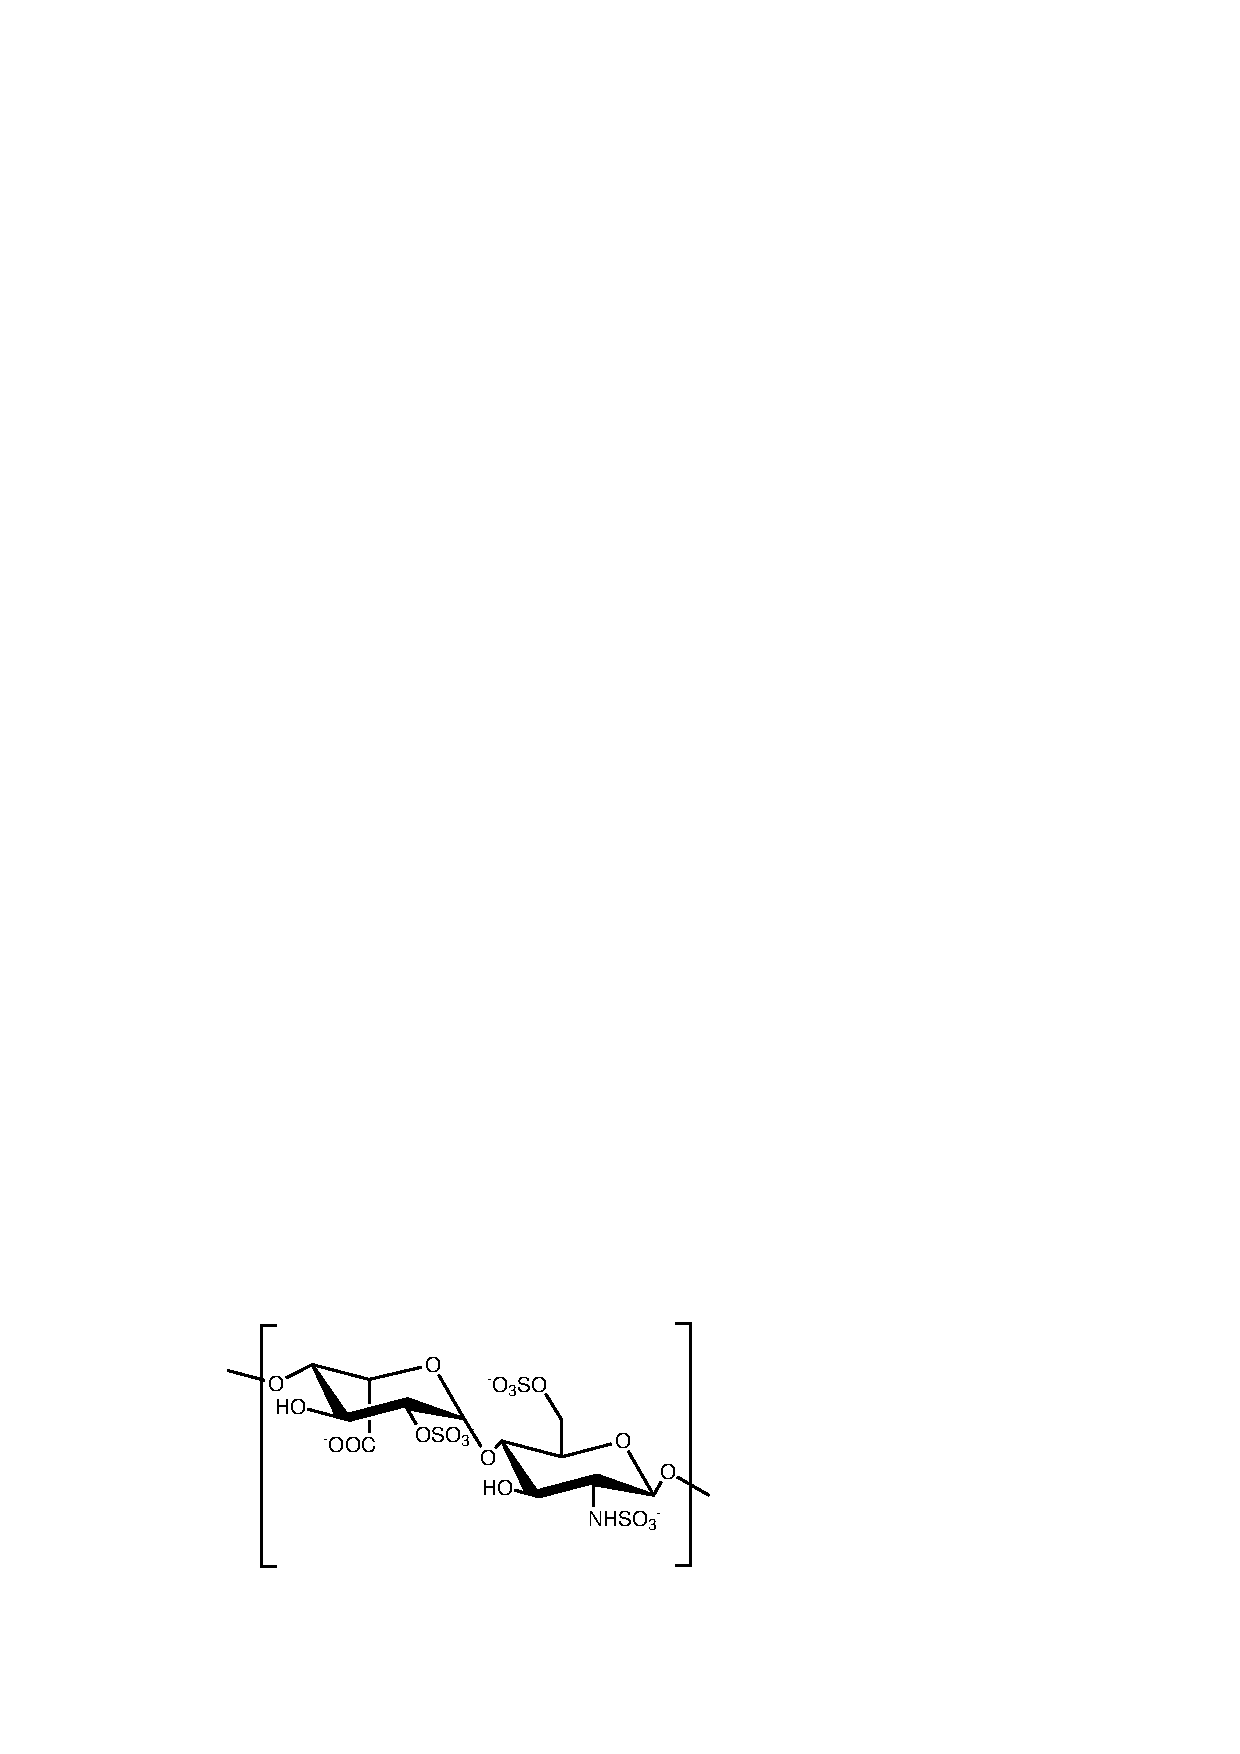
\includegraphics[height=3cm]{Heparin.jpg}
% \caption{\cmpd{Heparin}}
% \end{subfigure}%
% \begin{subfigure}{.5\textwidth}
% \centering
% 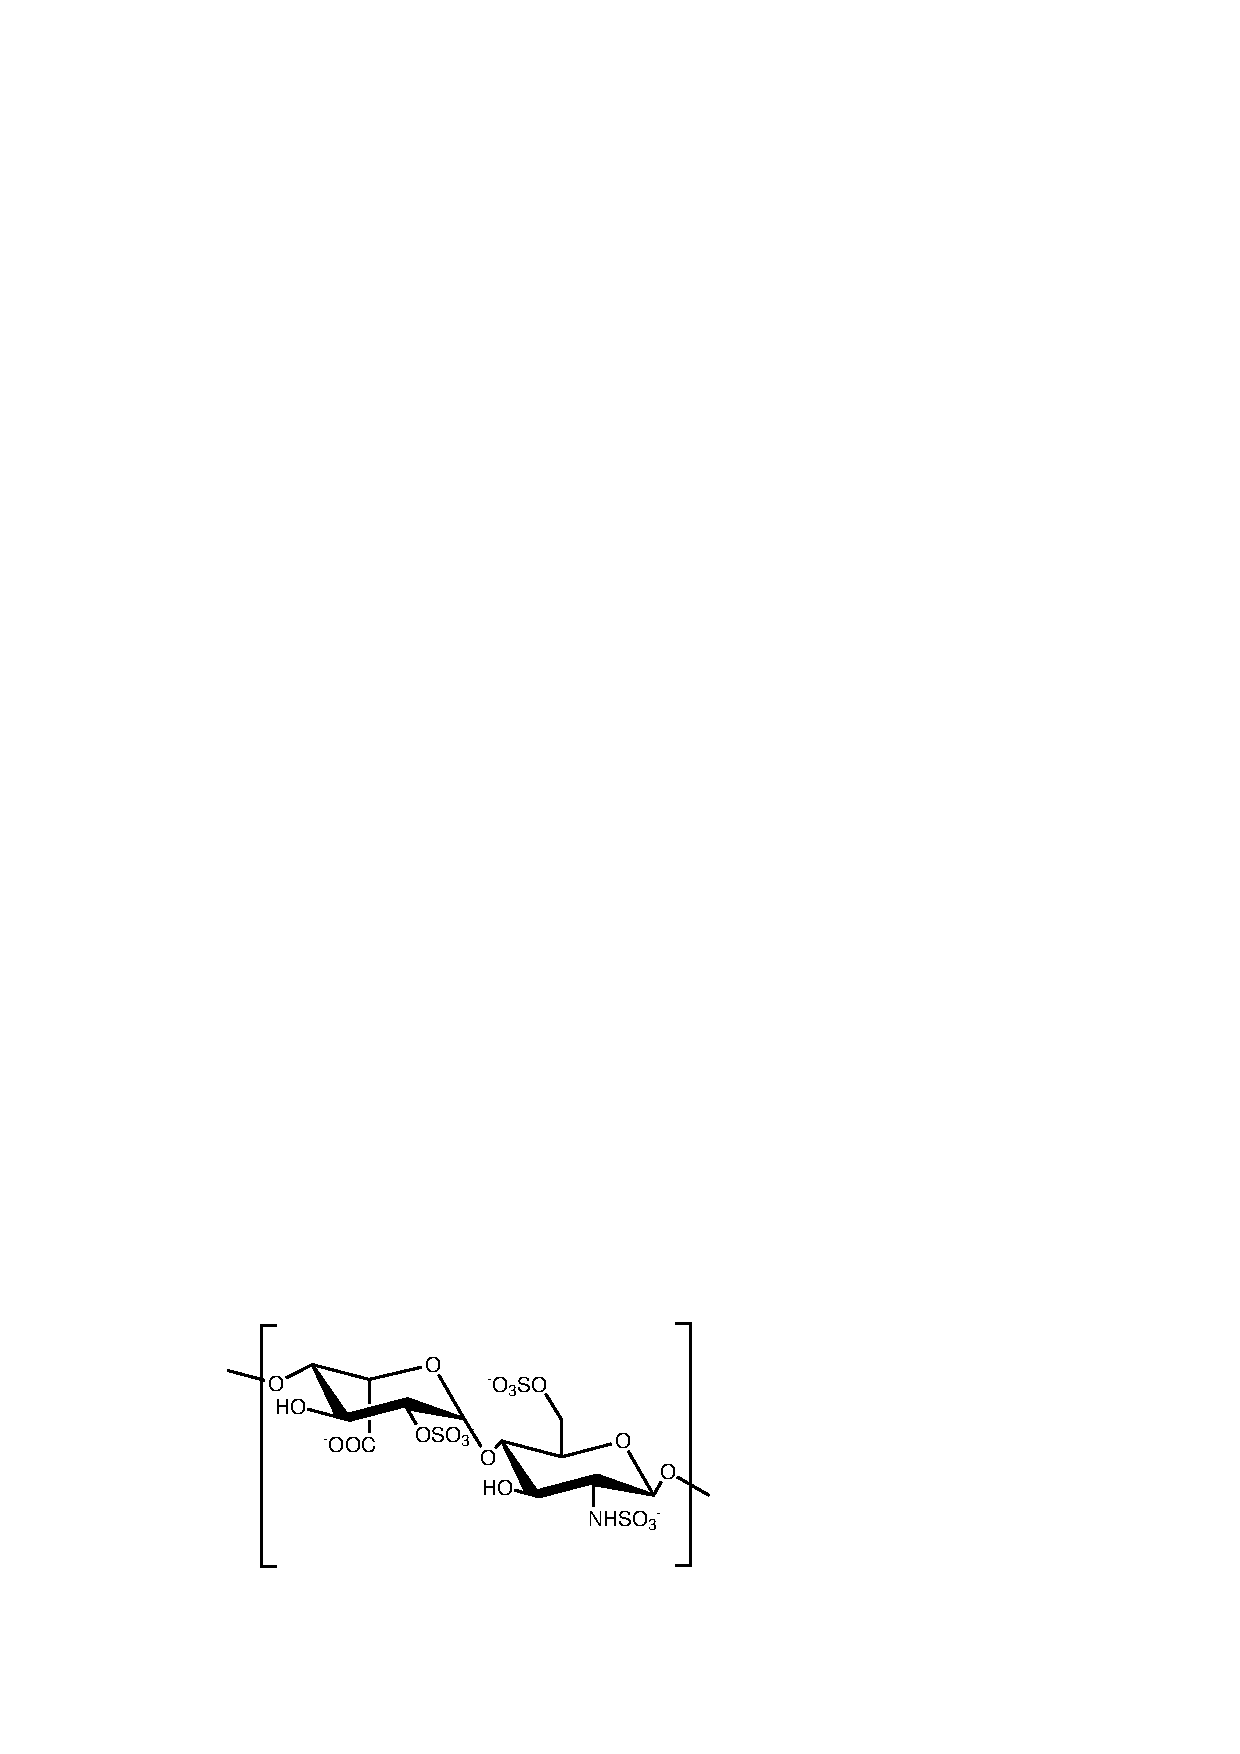
\includegraphics[height=3cm]{Heparin.jpg}
% \caption{Test subfigure 2}
% \end{subfigure}%
% \caption{Two subfigures}
% \end{figure}

\afterpage{
\begin{table}[H]
\begin{tabular}{m{5em}m{12em}m{5em}m{12em}} \hline \hline
    GAG & Major repeating units & Possible Sulfation & Features \tabularnewline \hline \hline
    Heparin (Hep) & \vspace{1mm}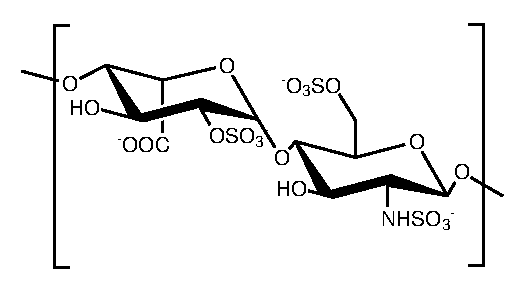
\includegraphics[width=5cm]{structures/Heparin.eps} {\small L}-Ido2S-\textalpha(1\textrightarrow4)-{\small D}-GlcNS \vspace{1mm} &\textbf{GlcNS:}\newline 3S, 6S & \Ac{DoS}: \tabularnewline
    Heparan sulfate (HS) & \vspace{1mm}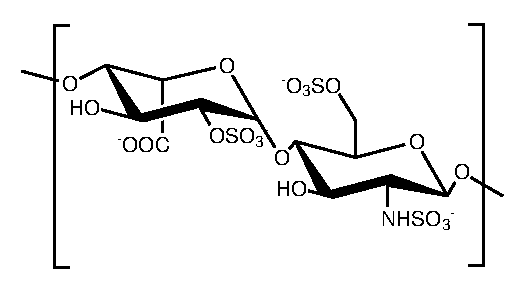
\includegraphics[width=5cm]{structures/Heparin.eps} {\small L}-Ido2S-\textalpha(1\textrightarrow4)-{\small D}-GlcNS \vspace{1mm}& \textbf{GlcA:}\newline 2S \newline \textbf{GlcNS:}\newline 3S, 6S &
    \tabularnewline
    \hline

    Hyaluronic acid (HA) & \vspace{1mm}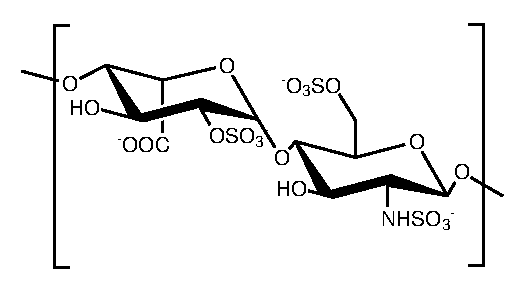
\includegraphics[width=5cm]{structures/Heparin.eps} {\small L}-Ido2S-\textalpha(1\textrightarrow4)-{\small D}-GlcNS \vspace{1mm}& &
    \tabularnewline
    \hline

    Chondrodin sulfate (CS) & \vspace{1mm}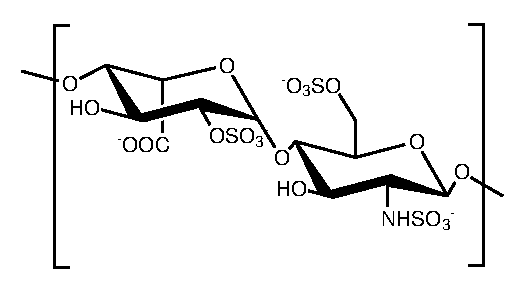
\includegraphics[width=5cm]{structures/Heparin.eps} {\small L}-Ido2S-\textalpha(1\textrightarrow4)-{\small D}-GlcNS \vspace{1mm}& \newline \textbf{GlcNAc:}\newline4S, 6S \newline 4S6S \newline \textbf{GlcA:}\newline 2S &
    \tabularnewline
    Dermatin sulfate (DS) & \vspace{1mm}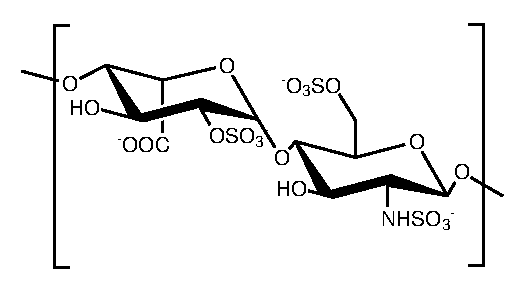
\includegraphics[width=5cm]{structures/Heparin.eps} {\small L}-Ido2S-\textalpha(1\textrightarrow4)-{\small D}-GlcNS \vspace{1mm}& \textbf{GlcNAc:}\newline4S &
    \tabularnewline
    \hline
    
    Keratan sulfate (CS) & \vspace{1mm}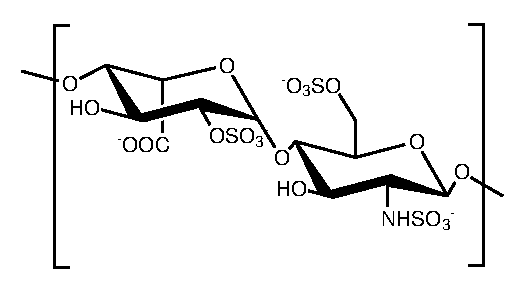
\includegraphics[width=5cm]{structures/Heparin.eps} {\small L}-Ido2S-\textalpha(1\textrightarrow4)-{\small D}-GlcNS \vspace{1mm}&
    \textbf{Gal:}\newline6S \newline \textbf{GlcNAc:}\newline6S &
    \tabularnewline
    \hline
    
\end{tabular}
    \caption{The structures and features of glycosaminoglycans, including reported \ac{DoS}.}
    \label{tab:my_label}
\end{table}
}

\subsubsection{Function}

\Acp{GAG} are present in the extracellular matrix \ac{ECM} of all animal cells, found on the surface and in solution. These sugars bind to distinct attachment receptors on proteins such as chemokines, cytokines, growth factors, morphogens, enzymes and adhesion molecules\cite{Murphy2007StructuralHeparin, Iozzo2001HeparanArena, Kreuger2006InteractionsSpecificity, Kowitsch2018MedicalReview}. \ac{HS} and \ac{Hep} are key to the regulation of Alzheimer's  \textbeta-secretase (BACE1), as they bind to BACE-1 and inhibit cleavage of \ac{APP} and aggregate into amyloid plaques.\cite{Swarup2013SugarNeurons,Scholefield2003HeparanBeta-secretase.} Other GAG chains, including CS and DS, are also found within these plaques and may contribute to plaque formation and the overall progression of the disease. Previous research also showed that HS, CS, and KS can all interact with AB peptides and enhance the shift of AB42 peptides to the \textbeta-sheet confirmation. GAGs in solution can inhibit proteins that target specific GAG sequences on the surface of PGs, for example, a heparin pentasaccharide interacts with certain binding pockets on fibroblast-growth-factor 1 and 2 (FGF, FGF1, FGF2), blocking interactions with proteins associated with proteolysis, which proliferates the FGFs, causing morphological changes to the cell\cite{SoaresdaCosta2017SulfationDisorders}. 

GAG sulfation creates specific microenvironments at the ECM, which serves to direct the permeation of small cations, the proliferation of stem cells and the regulation of neuronal development in humans, amongst other processes. 

\subsubsection{Protein interactions}
Carbohydrates form hydrogen bonds with side chain residues of polar planar amino acid residues (ASN, ASP, GLY, GLN, ARG and HIS)\cite{Malik2007SequenceNetwork}.
These hydrogen bonds can be cooperative hydrogen bonds, bidentate hydrogen bonds or hydrogen bond networks and facilitate low energy conformations of the polysaccharide.\cite{Quiocho1989Protein-carbohydrateFeatures} 



\subsection{Computational methods and their roles in drug discovery}

`Big O'  notation, $\mathcal{O}(f(n))$, is a concept in computer science that relates the size of a task to the time taken to complete the task using a given algorithm. A task of $\mathcal{O}(n^{2})$ implies a quadratic relationship between the size of the task and the time taken to complete it.

\subsubsection{Quantum mechanics}
\Ac{QM}

\subsubsection{Molecular dynamics}
\Ac{md}

\subsubsection{Docking}

\subsubsection{Statistical methods}

The distribution of amino acid residues at carbohydrate binding sites suggests

\subsection{Current advances in GAG/carbohydrate docking}

\subsubsection{Cluspro: heparin sitemapping (2014)}

The Cluspro server is an online protein--protein docking package which was adapted in 2014 to include a tool used for \ac{Hep}/\ac{HS} site mapping tool.\cite{Comeau2007ClusPro:Server, Mottarella2014DockingProteins,Kozakov2017TheDocking.} 
Cluspro performs three main computational procedures: \ac{RBD}, \ac{RMSD} clusering and refinement using an energy minimization function.\cite{Kozakov2017TheDocking.} 

% The rigid body docking step uses PIPER16, a docking program based on the Fast Fourier Transform (FFT) correlation approach. The FFT approach, introduced by Katchalski-Katzir and co-workers17 in 1992, led to major progress in rigid body protein-protein docking. In this method, one of the proteins (which we will call the receptor) is placed at the origin of the coordinate system on a fixed grid, the second protein (which we will call the ligand) is placed on a movable grid, and the interaction energy is written in the form of a correlation function (or as a sum of a few correlation functions). The numerical efficiency of the methods stems from the fact that such energy functions can be efficiently calculated using Fast Fourier Transforms, and results in the ability of exhaustively sampling billions of the conformations of the two interacting protein, evaluating the energies at each grid point. Thus, the FFT based algorithm enables docking of proteins without any a priori information on the structure of the complex. Katchalski-Katzir et al.17 used a simple scoring function that accounted only for shape complementarity. However, subsequent methods based on the FFT correlation approach to docking introduced more complex and more accurate scoring functions that also included terms representing electrostatic interactions18,19, or both electrostatic and desolvation contributions20. A key to the success of rigid body methods is that the shape complementarity term allows for some overlaps, and hence the methods are able to tolerate moderate differences between bound and unbound (separately crystallized) structures. As will be discussed, one of the distinguishing characteristics of PIPER, the docking program used in the current version of ClusPro, is that this implementation of the FFT correlation method employs a scoring function that includes a structure-based pairwise interaction term, and the combination with the other terms in the energy function substantially increases the accuracy of docking, resulting in more near-native structures16.

%The second step performed by ClusPro is clustering the retained structures using pairwise RMSD as the distance measure.37 The biophysical meaning of clustering is isolating highly populated low-energy basins of the energy landscape.38 Several studies, including ours,31 have demonstrated that clustering algorithms generally perform better for isolating near native structures as compared with selecting low-energy conformations, if used in conjunction with exhaustive energy-based sampling such as in PIPER.

\subsubsection{VinaCarb (AutoDock Vina) (2016)}
\ac{RMSD}
\ac{PRMSD}

\subsubsection{GAG--Dock (DarwinDock/GenDock) (2017)}
The ``GAG-Dock" method reported by
\citeauthor{Griffith2017PredictingGrowth}\cite{Griffith2017PredictingGrowth} was developed using DarwinDock and GenDock to model GAG--protein interactions. This method accurately predicted \ac{Hep} binding poses within 0.70 - 1.51 \r{A} \ac{RMSD} of the crystal structures (\ac{FGF1}, \ac{FGF2}, and \ac{AT3}. The authors also investigated the specificity of protein binding, through in silico mutations, to favor a particular GAG sulfation pattern. 
To establish the available space for a ligand to dock, a modified version of the sphgen program\cite{Moustakas2006Development5} was used. Sphgen generates concentric spheres that combine to form a curve topology which is used to model the surface of the protein. 
Sphgen can also be used to analysing clustering of docked ligands.\cite{Hendrix1998SurfaceDocking.}
To model \ac{GAG} binding to flat surface, the available space for ligands to bing to flat protein surfaces was increased. In this modification, the “dotlim” parameter in sphgen was altered. The default ``dotlim" value, zero, prevents generation of large spheres with close surface contacts.\cite{Hendrix1998SurfaceDocking.} For \acp{GAG} ``dotlim" parameter was decreased to - 0.9, which allowed for spheres to be generated for flat surfaces.\cite{Griffith2017PredictingGrowth} To prevent sampling from pockets inside the protein that would be inaccessible to \asp{GAG}, a two sphere surfaces are generated by using the normal probe radius the normal 1.4 \r{A} and a larger radius of 2.8 \r{A}. The intersection of these surfaces is taken to generate spheres on the protein surface without sampling from too close to, or outside of, the surface.\cite{Griffith2017PredictingGrowth} 

\subsection{Current challenges in glycosaminoglycan docking}


\section{Aims}

\section{Methods}


}
\newpage
{\setstretch{0}
\bibliography{mendeley_v2}
}
\newpage
\section{Appendix}
\end{document}

